%!TEX program = pdflatex
\documentclass{article}

% Opening
\title{
	   Programación Dinámica: Transferring Pyramids\\
	   \texttt{{\large (https://codeforces.com/problemset/problem/354/D)}}}
\author{Carlos Luis Aguila Fajardo}
\date{}

% Packages
\usepackage{amsmath}
\usepackage{amsthm}
\usepackage{amssymb}
% \usepackage{relsize}
\usepackage[utf8]{inputenc}
% \usepackage{wrapfig}
\usepackage{tikz}
\usetikzlibrary{positioning}
\usetikzlibrary{matrix}
\usetikzlibrary{patterns}

% Teoremas, demostraciones, proposiciones, lemas y definiciones
\newtheoremstyle{default}
	{\topsep}
	{\topsep}
	{}
	{0pt}
	{\bfseries}
	{:}
	{4pt plus 1pt minus 1pt}
	{}
\theoremstyle{default}
\newtheorem{theorem}{Teorema}
\newtheorem*{theorem*}{Teorema}
\newtheorem*{lemma}{Lema}
\newtheorem*{note}{Nota}
\newtheorem*{proposition}{Proposición}
\newtheorem*{demonstration}{Demostración}
\newtheorem*{definition}{Definición}
\newtheorem{property}{Propiedad}
\begin{document}
\maketitle
%
%
%
\section{Problema}
	\subsection{Analogía}
		El problema requiere, dada una estructura de datos planteada y las operaciones con costo definidas, encontrar el costo mínimo de las operaciones que `arregle' los valores iniciales modificados en la estructura.
		\subsubsection{Estructura utilizada}
			La estructura de datos planteada en el problema puede ser compleja para explicar su solución. Dada su naturaleza tan específica, el equivalente de mayor facilidad relativa para representarla es un arreglo bidimensional escalonado, o bien una matriz triangular inferior. Formalmente, se tiene una matriz $M \in M_{n \times n}$ triangular inferior, tal que en cada columna $i$, se tienen exactamente $i$ elementos, y en cada fila $j$ se tienen exactamente $n-j+1$ elementos, de la forma:
			%
			\begin{equation*}
				m_{ij} \in M, \quad \forall i,j: 1 \leq j \leq i \leq n
			\end{equation*}
			%
			que puede visualizarse de la siguiente forma:
			%
			\begin{center}
				\begin{tabular}{|*4{c|}}
					\cline{1-1}
					$m_{n,n}$ \\
					\cline{1-2}
					$$\vdots$$	& $\ddots$	\\
					\cline{1-3}
					$m_{n,2}$  	&			& $m_{2,2}$  	\\
					\hline
					$m_{n,1}$	& $\dots$	& $m_{2,1}$ 	& $m_{1,1}$	\\
					\hline
				\end{tabular}
			\end{center}
			%
			% \begin{center}
			% 	\begin{tabular}{|*4{c|}}
			% 		\cline{1-1}
			% 		$m_{1,1}$ \\
			% 		\cline{1-2}
			% 		$m_{1,2}$	& $m_{2,2}$	\\
			% 		\cline{1-3}
			% 		$\vdots$  	& $\vdots$	& $\ddots$  \\
			% 		\hline
			% 		$m_{1,n}$	& $m_{2,n}$	& $\dots$	& $m_{n,n}$	\\
			% 		\hline
			% 	\end{tabular}
			% \end{center}
			Nótese los cambios realizados por comodidad de notación e implementación, contrario al convenio de matrices, el primer subíndice indica la columna del elemento (enumeradas de derecha a izquierda), el segundo su fila en términos de altura (es decir, enumeradas de abajo hacia arriba).

			De usarse el concepto como matriz, los elementos $m_{ij}$ donde $j > i$ no son de importancia pues nunca son utilizados bajo las circunstancias del problema; bien puede considerarse $m_{ij} = \infty, \forall j > i$ o utlizar una estructura similar a una matriz irregular o \textit{jagged array}, en que solo se mantienen filas o columnas del tamaño adecuado.
	%
		\subsubsection{Definiciones y propiedades de la estructura}
			\begin{definition}
				Llamaremos $P \in P_n$ una pirámide a la estructura que cumpla lo anteriormente mencionado. Por formalidad se utilizará poco el término pirámide, solo de ser necesario para desambiguar una estructura a la que se haga referencia.
			\end{definition}
			%
			\begin{definition}
				Los valores $m_{ij}$ que pertenecen a la matriz con $j \leq i$ serán de la forma $m_{ij} = 1$ si el valor en la posición $(i,j)$ fue modificado, dígase, es un cambio, sino tomará valor $0$ en el caso contrario.
			\end{definition}
			%
			\begin{definition}
				Sea $P \in P_n$, llamaremos $P(m_{ij})$ la subpirámide o matriz inducida de $P$ con tope o que inicia en $m_{ij}$, que cumple:
				\begin{equation*}
					P(m_{kh}) \in P_{h}
				\end{equation*}
				\begin{equation*}
					\forall i,j:\ 1 \leq j \leq h,\ j+(k-h) \leq i \leq k: m_{ij} \in P(m_{kh})
				\end{equation*} 

			\end{definition}
			%
			\paragraph{}De estas estructuras se pueden deducir ciertas propiedades de utilidad para demostraciones posteriores.
			%
			\begin{property}
				$P \in P_n$ tiene exactamente $\frac{n(n+1)}{2}$ elementos.
			\end{property}
			\begin{demonstration}
				Por definición $P$ tiene $n$ columnas y filas, y por cada columna tiene exactamente $i$ elementos. Entonces:
				\begin{equation*}
					\sum\limits_{i=1}^{n}{i} = \frac{n(n+1)}{2}
				\end{equation*}
			\end{demonstration}
			\begin{property}\label{no-left-column-property}
				Sea $P \in P_n, P(m_{kh})$ no cubre ningún $m_{ij}: i > k$.
			\end{property}
			\begin{demonstration}
				Por consecuencia directa de la definición podemos ver que todo $i$ en $m_{ij} \in P(m_{kh})$ debe cumplir $i \leq k$.
			\end{demonstration}
	%
		\subsubsection{Operaciones permitidas. Definición formal.}
			En el problema se definen dos operaciones posibles.
			%
			\begin{enumerate}
				\item Cambiar un valor $m_{ij}$ con costo $3$.
				\item Cambiar $P(m_{ij})$, de tamaño $i$, con costo $\frac{n(n+1)}{2} + 2$. Es válido que solo sea necesario cambiar algunos elementos dentro de $P(m_{ij})$, por lo que se pueden mantener los valores idénticos del resto, pero el costo no se reduce aunque esto ocurra.
			\end{enumerate}
	%
\section{Demostraciones de utilidad}
	\begin{lemma}
		Sea $P \in P_{n}$, $P(m_{kh})$ no cubre todos los $m_{ij}: i \leq k$ a no ser que $k = h$.
	\end{lemma}
	\begin{demonstration}
		Conocemos por definición que nunca ocurre que $k < h$, entonces si ocurre que $k \neq h$ necesariamente $k > h \implies k - h > 0$. Adicionalmente, todo $m_{ij} \in P(m_{kh})$ cumple:
		%
		\begin{align*}
			j + (k-h) &\leq i \leq k				\\
			j + (k-h) &\leq i						\\
			j 		  &< 	i - (k-h) + 1, \quad k-h > 0
		\end{align*}
		%
		entonces $\forall i,j^\prime: j^\prime \in [i - (k-h) + 1, i\,]: m_{ij^\prime} \notin P(m_{kh})$. Sin pérdida de generalidad, podemos establecer la cantidad de elementos cubiertos por el intervalo:
		\[
			i - (i - (k-h) + 1) + 1 \ = \ k - h
		\]
		por tanto siempre existen para todo $i$ una cantidad $k - h$ de diagonales no cubiertas, que bien puede ser $0$ de ocurrir $k = h$. Por ejemplo, en la siguiente figura, $P(m_{4,2})$ no cubriría $k-h=2$ diagonales, las coloreadas.
		%
		\begin{center}
			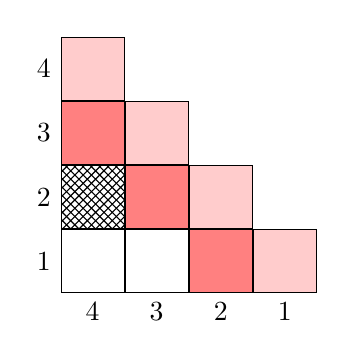
\begin{tikzpicture}
				\matrix (A) [
					matrix of nodes, nodes={draw, minimum size=8mm}, nodes in empty cells
				]{
					|[fill=red!20]|		\\
					|[fill=red!50]| 	& |[fill=red!20]|	\\
					|[pattern=crosshatch]|& |[fill=red!50]| 	& |[fill=red!20]|	\\
					||&	||& |[fill=red!50]| 	& |[fill=red!20]|	\\
				};
				
				\node also [pattern=north east lines] (A-1-1) {};

				\foreach \i [count=\xi from 1] in {4,...,1} {
					\node also [label=below:\xi] (A-4-\i) {};
					\node also [label=left:\xi] (A-\i-1) {};
				};
			\end{tikzpicture}
		\end{center}
	\end{demonstration}
	\begin{proposition}
		Utilizando los resultados de la \textbf{Propiedad \ref{no-left-column-property}}, se puede observar que sea $P(m_{kh}), k \neq n$, intuitivamente existen $n - k$ columnas no cubiertas por esta.
	\end{proposition}
	\begin{theorem}
		El costo total de resolver cierta $P \in P_n$ utilizando $p = P(m_{kh})$ es el costo de insertarla, más:
		\begin{enumerate}
			\item si $h \neq k$, el costo que haya tomado resolver las $k - h$ diagonales que no haya cubierto $p$.
			\item si $h \neq n$, el costo de resolver los elementos $\{m_{k,h+1}, \dots m_{k,n}\}$ restantes de la columna $k$.
			\item si $k \neq n$, el costo de resolver, si existen, las columnas $i \geq k$.
		\end{enumerate}
	\end{theorem}
	\begin{demonstration}
		Los costos 1 y 3 son consecuencias directas de las demostraciones anteriores. Respecto al segundo punto, fue separado por facilidad de demostración posterior. Es fácil ver que si no se consideran esos elementos $\{m_{k,h+1}, \dots m_{k,n}\}$ como parte de las diagonales, son costos adicionales a tener en cuenta durante una solución.
	\end{demonstration}	
	%
%
\section{Solución}
	\subsection{Planteamiento recursivo}
		Sea $P \in P_n$, supongamos que se tienen, para la columna $n$, los costos de resolver todas las diagonales desde $i-\alpha$ hasta $i$. Hallar el costo mínimo de resolver el problema se reduciría a:

		Por cada altura $h$ desde $1$ hasta $n$, considerar el costo de insertar $P(m_{n,h})$, más el de resolver las $n-h$ diagonales restantes, más el de resolver los elementos de altura mayor que $h$ restantes en la columna. No sería necesario resolver columnas restantes pues $n$ es la última columna. Sea $c(x)$ la función de costo:
		%
		\begin{equation}
			\label{subpyramid_costs}
			c(P) = c(P(m_{n,h})) + \sum\limits_{i=h+1}^{n}{c(m_{n,i})}
								 + \sum\limits_{t=1}^{k-h}{c\Big(
										\Big\{m_{i,j} \, | \ j=i-t,\ i < n \Big\}\Big)}
		\end{equation}
		%
		De esta forma se puede considerar un paso recursivo donde aplicar esta lógica en cualquier $P(m_{l,l})$ permite, asumiendo que podemos generar los costos de las diagonales, no tener que resolver el costo de las columnas mayores que $l$.
		%
		\subsubsection{Equivalencia respecto a las diagonales}
			Es posible replantear el problema de los costos de las diagonales como, al considerar la $k$-ésima columna, por cada altura $h$ determinar cual es el costo mínimo de solucionar la columna actual asumiendo que los valores de $[1,h]$ están ya resueltos.

			De esta forma por cada altura $h$ de la columna se tendría el costo acumulado de las diagonales que pasan entre $h$ y $n$ por la columna actual.
		
	%
	\subsection{Formalización como algoritmo dinámico}
		Sea $dp$ un arreglo de columnas tal que $\forall h,k: 0 \leq h \leq k: dp[k][h]$ define el menor costo de solucionar la columna $k$ asumiendo que los elementos de $[1,h]$ ya tienen solución mediante la inserción de una subpirámide en alguna columna mayor que $k$ que cubra a $h$.

		Sin embargo, $dp[k][0]$ resulta un caso especial, para hallar el mínimo costo de solucionar los cambios presentes en la columna $k$, asumiendo que no existe solución 
		en otra columna que lo cubra, sería intuitivo probar a fuerza bruta todas las posibles subpirámides que se puedan insertar en filas o alturas $[1,k]$, además de que pueden existir casos en que sea mejor no insertar ninguna y cubrir los cambios en la columna uno a uno con costo individual $3$.

		Definimos entonces el caso especial para $0$ y luego para cualquier $k \geq 1$.
		%
		\begin{align}
			\nonumber
			dp[k][0] = \min & \Bigg(
						dp[k-1][0]
					  	+ 3 \cdot \sum\limits_{i=1}^{k}{(m_{k,i})},
			\\
			\label{dp_0_all}
					 	&\min_{\forall i \in [1,k]} \biggl(
						dp[k-1][i-1] + c(P_i) + 3\cdot\!\sum\limits_{j=i-1}^{k}(m_{k,j})
					\biggr)\Bigg)
		\end{align}
		Podemos observar que, al tratarse en $dp[k][0]$ con todas las posibles inserciones en la columna, el mínimo en cada iteración depende de la columna anterior de $dp$ en su totalidad, pues en ella se encuentra la información de todas las posibles diagonales que pasan por la columna $k$, y por tanto $dp$ minimiza los resultados no solo de la actual, sino de todo mínimo que haya sido procesado a su derecha, donde cubrirían sus inserciones.

		Con esto garantizamos que en $dp[k][0]$ siempre se encuentra la solución para una matriz $P_k$, por lo tanto la solución final del problema se encontraría en $dp[n][0]$. Dada la dependencia de este sobre las columnas anteriores, sería correcto asumir que $dp[k][h], h \neq 0$ solo contiene información de utilidad para computaciones posteriores, no es de interés como respuesta final del problema, y por tanto no sería siquiera necesario computar estos valores en la última columna.

		Dada su existencia como historial de los óptimos parciales de las diagonales, la expresión para computar los $dp[k][h]$ resulta mas simple a primera vista:
		%
		\begin{equation}
			\label{dp_h_all}
			dp[k][h] = \min_{\forall i \in [1,k]} \left(
				dp[k][i-1], \ dp[k-1][i-1]
				+ 3 \cdot \sum\limits_{j=i-1}^{k}m_{k,i}
				\right)
		\end{equation}
		%
		Nótese que la parte izquierda mantiene referencia a la respuesta inmediatamente anterior de la columna, porque puede ocurrir que una inserción encontrada por $dp[k][0]$ sea mejor que la respuesta parcial de la diagonal hasta el momento.
		
		\paragraph{}Finalmente, como $dp$ depende exclusivamente de computaciones de la columna anterior y de la actual, podemos rellenarlo ascendientemente por columnas de derecha a izquierda. Es de utilidad predefinir $dp[0][0] = 0$ a pesar de no existir una columna $0$, por cubrir el caso base dentro del propio ciclo sin tener que computar a mano la primera columna.
	%
	\subsection{Complejidad temporal}
		El algoritmo recorre $n+1$ columnas de a lo sumo $n+1$ elementos. La unión de las iteraciones de $dp[k][0]$ y $dp[k][i]$ no superan las $2(n+1)$ iteraciones, sin embargo se realiza una suma $O(n)$ por iteración.

		Como consecuencia de esto se tiene un algoritmo $O(n^3)$. Si optimizamos el cálculo de las sumas ascendentes mediante el uso de sumas de prefijos (\textit{prefix sums}) entonces por cada columna se procesan una sola vez las sumas y se almacenan en un arreglo accesible en $O(1)$, lo que terminaría reduciendo la complejidad temporal de nuestro algoritmo a $O(n^2)$.
	%
	\subsection{Optimizaciones de complejidad temporal}
		Conocemos que el costo de arreglar celdas independientes de la matriz es de 3. Sea $k$ la cantidad de cambios iniciales de entrada a arreglar, ha de existir una subpirámide lo suficientemente grande como para ser siempre peor que simplemente modificar los $k$ elementos a un costo total de $3k$. Busquemos el valor $n$ a partir del cual se cumple, para $k$ de entrada arbitrario, que:
		\begin{align*}
			3k 			& \leq \frac{n(n+1)}{2} 	< \frac{(n+1)^2}{2}	\\
			3k 			& < \frac{(n+1)^2}{2}							\\
			\sqrt{6k} 	& < n + 1										\\
			\sqrt{6k}	& \leq n
		\end{align*}
		%
		Entonces no tiene sentido intentar insertar una subpirámide de altura $h \geq \sqrt{6k}$. Podemos realizar por tanto modificaciones en el cálculo de sumas y la iteración interna de las columnas para que no supere dicha cota. De forma que podemos mejorar la complejidad temporal del algoritmo a $O(n\sqrt{k})$.
		%
	%
	\subsection{Optimizaciones de complejidad espacial}
		Como se puede observar en (\ref{dp_0_all}) y (\ref{dp_h_all}), $dp$ solo depende de los valores de la columna inmediatamente anterior y la actual, por lo tanto podemos reducir el tamaño de $dp$ a un arreglo $2 \times n$ e ir intercambiando las referencias entre la columna `actual' y la `anterior'. De esta forma la complejidad espacial del algoritmo termina siendo $O(n)$.
	%
\section{Implementación y comprobación de casos}
	En el archivo \texttt{scripts/pyramid.py} se encuentra la implementación de la versión no mejorada del algoritmo. La versión mejorada en complejidad algorítmica y espacio de memoria se encuentra en \texttt{scripts/pyramid\_opt.py}.
	
	Por las especificidades del problema, no estuvo en mi capacidad encontrar una forma mediante fuerza bruta de obtener la solución, considerando que el algoritmo sin optimización en sí es casi una forma de hacerlo por fuerza bruta.

	En lugar de verificar la correctitud del algoritmo utilizando otro mas básico, que es lo ocurrido en otros problemas, fue implementado un comparador, que se encarga de verificar que tan rápido es el algoritmo mejorado respecto al básico. Por esta razón se permite en el código generador que el tamaño de los datos de prueba sea un poco mas grande que en otros problemas, para mostrar diferencias de tiempo evidentes.

	Por la dificultad de Python para verificar uso de memoria sin el uso de librerías externas, la comparación es realizada solo en tiempo de ejecución.

	\subsection{Generación de casos}
		Similarmente a otros problemas, la generación de casos para realizar estas verificaciones es en gran parte aleatoria. Se elige un $n$ la altura de la pirámide, y se crean cambios en la posición $(c,r)$, columna y fila respectivamente, aleatorias, donde se cumple que $c \leq r$.
%
%
%
\end{document}